146. \begin{figure}[ht!]
\center{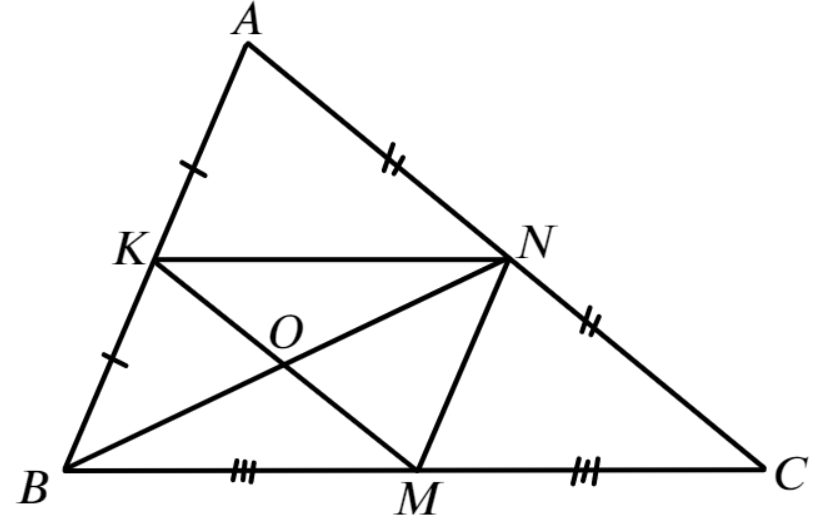
\includegraphics[scale=0.35]{g9-146.png}}
\end{figure}\\
Средняя линия параллельна основанию, значит $BKNM$ является параллелограммом. Треугольник $BKM$ подобен треугольнику $ABC$ по двум углам (соответственным) с коэффициентом $\cfrac{KM}{AC}=\cfrac{1}{2},$ значит $S_{\Delta BKM}=\cfrac{1}{4}S_{\Delta ABC}.$ Тогда $S_{\Delta OMN}=\cfrac{1}{2}S_{\Delta KMN}=\cfrac{1}{2}\cdot\cfrac{1}{4}S_{\Delta ABC}=\cfrac{1}{8}S_{\Delta ABC}.$\\
